\documentclass[12pt]{exam}
\usepackage{graphicx} % Required for inserting images
\usepackage{amssymb}
\usepackage{amsmath}
\usepackage{optidef}
\usepackage{listings}
\usepackage{xcolor} % for custom colors
\usepackage{minted} % for code

\lstset{
  language=Python,
  basicstyle=\ttfamily\small,
  keywordstyle=\color{blue},
  stringstyle=\color{red},
  commentstyle=\color{gray},
  showstringspaces=false,
  frame=single,
  breaklines=true
}
\title{15.051 Mathematical programming, HW2}
\author{Erich Trieschman}
\date{2025.10.02}
\begin{document}
\maketitle

\begin{questions}
    \question \textbf{3.9 Necessary and sufficient conditions for global optimum}

    \textbf{Given:} Linear problem in standard form, $\min_x c^Tx \quad \text{s.t.} \; Ax=b, \; x \geq 0$ and $x^*$ optimal. $B, N=B^C$ the sets of basic and nonbasic indices of the optimal basis for $x^*$. $I \in N$ such that $\Bar{c}_i = 0$ for $i \in I$
    \begin{parts}
        \part \textbf{Show:} $I$ empty $\Rightarrow x^*$ only optimal solution

        \textbf{Contradiction:} Suppose $\exists\; y^* \neq x^*$ s.t., $c^T y^* = c^T x^*$, a distinct second optimal solution. We can define search direction $d = y^* - x^*$. Since $y^*, x^*$ optimal BFS, we have 
        \begin{align*}
           0 &= Ay^* - A x^* = Ad = \sum_{i\in B} A_{B(i)}d_{B(i)} + \sum_{j \in N} A_{N(j)}d_{N(j)} = Bd_B + Nd_N\\
           d_B &= -B^{-1}Nd_N
        \end{align*}
        Now the cost improvement vector is
        \begin{align*}
            0 &= c^T(y^* - x^*) = c^Td = c_B^Td_B + c_N^Td_N\\
            &= c_N^Td_N - c_B^TB^{-1}Nd_N = \big(c_N^T - c_B^TB^{-1}N\big) d_N\\
            &:= \bar c_N^Td_N
        \end{align*}
        Now from what we know,
        \begin{align*}
            x_N = 0 & \Longrightarrow d_N = y^*_N - x^*_N = y^*_N\\
            y^*_N \text{ optimal solution }&\Longrightarrow y^*_N \geq 0 \Longrightarrow d_N \geq 0\\
            x^* \text{ optimal} &\Longrightarrow \bar c_N \geq 0\\
            (I = \varnothing) \cup (\bar c_N \geq 0) &\Longrightarrow \bar c_N > 0\\
            (\bar c_N > 0) \cup (d_N \leq 0) \cup (\bar c_N^Td_N = 0) & \Longrightarrow d_N = 0
        \end{align*}
        So for optimal solution $y^* \neq x^*$, there is no change in direction $d_N$. But we also know that $Nd_N = 0 \Longrightarrow Nd_N = -Bd_B = 0$. Since $B$ invertible, it has a unique solution to $-Bd_B = 0\Longrightarrow d_B = \mathbf{0}$.

        Hence $d = [d_B, d_N] = \mathbf{0} \Longrightarrow 0 = y^* - x^* \Longrightarrow y^* = x^*$. Contradiction

        
        \part \textbf{Show:} $x^*$ only optimal solution $\iff \quad \sum_{i\in I} x_i=0$ in the below problem
        \begin{align*}
            \max &\quad \sum_{i\in I} x_i\\
            \text{s.t.}&\quad Ax=b\\
            &\quad x_i = 0 \text{ for } i \in N \setminus I\\
            &\quad x_i \geq 0 \text{ for } i \in B\cup I
        \end{align*}
        \begin{subparts}
            \subpart $\Longrightarrow:$ \textbf{(Contradiction)} Let $y$ be any feasible point s.t. $\sum_{i\in I} y_i > 0$. Since it is a feasible solution, we know $Ay = b$ and $y \geq 0$. 
            \newline\newline Define $d = y - x^*$. $Ad = 0 \Longrightarrow d$ is a feasible direction
            \newline\newline From part a), we have $c^Ty - c^T x^* = \bar c_N^Td_N$. Since $x^*$ optimal $\Longrightarrow c^Ty \geq c^T x^* \Rightarrow \bar c_N^Td_N \geq 0$
            \newline\newline Since $x_N = 0 \Longrightarrow d_N = y_N$. Now, from our supposition, $\exists\;i\in I$ such that $y_i > 0 \Longrightarrow d_i > 0$. By definition of $I$, the corresponding $\bar c_i = 0$.  And to be feasible in our axillary problem (i.e., $x_i = 0$ for $i \in N\setminus I$), we must have $y_{N\setminus I} = d_{N\setminus I} = 0$.
            \newline\newline Therefore, $0 = \bar c_N^T d_N = c^Ty - c^Tx^* \Longrightarrow c^Ty = c^Tx^*$. Contradiction to $x^*$ being the only optimal solution
            \newline
            \subpart $\Longleftarrow:$ \textbf{(Contrapositive)} Suppose $x^*$ is not the only optimal solution, then we show solution to the auxillary problem is $\sum_{i\in I} x_i>0$. 
            \newline\newline Given:
            \begin{itemize}
                \item $x^*$ not unique optimal $\Longrightarrow \exists$ feasible $y\neq x^*$ such that $c^Ty = c^Tx^*$
                \item Part a) by contrapositive: $x^*$ not unique optimal $\Longrightarrow I \neq \emptyset \Longrightarrow \exists\; i\in I$ such that $\bar c_i = 0$
            \end{itemize}
            For $\theta d = y - x^*$ we know we can construct feasible $y$ from search direction $d$ with:
            \begin{itemize}
                \item $d_i = 1$
                \item $d_j = 0$ for $j \in I\setminus\{i\}$
                \item $d_B = -B^{-1}A_i$
            \end{itemize}
            Such $d$ is a valid search direction since 
            \begin{align*}
                Ad = \sum_{j\in B} A_{B(j)}d_{B(j)} + \sum_{j \in N} A_{N(j)}d_{N(j)} = Bd_B + A_i = -BB^{-1}A_i + A_i = \textbf{0}
            \end{align*}
            so 
            \begin{align*}
                Ay = A(x + \theta d) = Ax + \theta Ad = Ax = b
            \end{align*}
            and $y$ is feasible for chosen $\theta = -\min_{\{i \in B \mid d_i > 0\}} \frac{x_i}{d_i}$, since $y = x + \theta d \geq 0$ for such a $\theta$.
            \newline\newline Now we have feasible $y$ with
            \begin{align*}
                0 &= c^T(y - x^*) = \theta c^Td\\
                &= (c^T_N - c^T_BB^{-1})Nd_n = \bar c^T_Nd_N \tag{see derivation in part a}
            \end{align*}
            since $\theta d_i > 0$ and $\theta d_{N\setminus \{i\}} = 0$ by construction $\Longrightarrow \bar c_i = 0 \Longrightarrow \{i\} \subseteq I \Longrightarrow \sum_{i\in I} y_i \geq \theta d_i > 0$
        \end{subparts}
    \end{parts}

    \question \textbf{3.12 Simplex implementation}
    
    \textbf{Given:}
    \begin{align*}
            \min &\quad -2x_1 - x_2\\
            \text{s.t.}&\quad x_1 - x_2 \leq 2\\
            &\quad x_1 + x_2 \leq 6\\
            &\quad x_1, x_2 \geq 0
    \end{align*}
    \begin{parts}
        \part Convert to standard form and construct BFS at $(x_1, x_2) = (0,0)$
        \begin{align*}
            \min &\quad -2x_1 - x_2\\
            \text{s.t.}&\quad x_1 - x_2 + x_3 = 2\\
            &\quad x_1 + x_2 + x_4 = 6\\
            &\quad x_1, x_2, x_3, x_4 \geq 0
        \end{align*}
        BFS: $(x_1, x_2, x_3, x_4) = (0, 0, 2, 6)$
        \part Carry out Tableau implementation of simplex, starting at BFS from part a
        \newline\newline Construct the initial Tableau matrix using
        \begin{align*}
            B = B^{-1} = \begin{bmatrix} 1&0 \\ 0&1 \end{bmatrix} 
            \quad A = \begin{bmatrix}1&-1&1&0\\ 1&1&0&1 \end{bmatrix}
            \quad b = \begin{bmatrix}2\\6\end{bmatrix}
            \quad c = \begin{bmatrix}-2 \\-1\\0\\0\end{bmatrix}
        \end{align*}
        Solve for quantities
        \begin{align*}
            -c_B^TB^{-1}b &= 0 \tag{since $c_B = \mathbf{0}$}\\
            c^T - c_B^TB^{-1}A &= c^T \tag{since $c_B = \mathbf{0}$}\\
            B^{-1}b &= b \tag{since $B^{-1} = I$}\\
            B^{-1}A &= A \tag{since $B^{-1} = I$}
        \end{align*}
        And we get Tableau
        \begin{align*}
            \begin{bmatrix}
               -c_B^TB^{-1}b &  c^T - c_B^TB^{-1}A\\
               B^{-1}b & B^{-1}A
            \end{bmatrix} = \begin{bmatrix}
                0 & c^T\\
                b & A
            \end{bmatrix} = \begin{bmatrix}
                0 & -2 &-1&0&0\\
                2 & 1 & -1 & 1 & 0\\
                6 & 1 & 1 & 0 & 1\\
            \end{bmatrix}
        \end{align*}
        \begin{table}[h!]
            \centering
            \begin{tabular}{rlcc}
            \hline
            \textbf{Step} && \textbf{Iteration 1} & \textbf{Iteration 2} \\
            \hline
            1.& Choose pivot column, $l$, based on $\bar c^T$ &
                $\begin{bmatrix}
                0 & -2 & \textcolor{red}{-1} & 0 & 0\\
                2 & 1 & \textcolor{red}{-1} & 1 & 0\\
                6 & 1 & \textcolor{red}{1} & 0 & 1\\
                \end{bmatrix}$ &
                $\begin{bmatrix}
                6 & \textcolor{red}{-1} & 0 & 0 & 1\\
                8 & \textcolor{red}{2} & 0 & 1 & 1\\
                6 & \textcolor{red}{1} & 1 & 0 & 1\\
                \end{bmatrix}$ \\
            2.& Choose pivot row, $i$, using ratio test & 
                $\begin{bmatrix}
                0 & -2 & \textcolor{red}{-1} & 0 & 0\\
                2 & 1 & \textcolor{red}{-1} & 1 & 0\\
                \textcolor{red}{6} & \textcolor{red}{1} & \textcolor{red}{1} & \textcolor{red}{0} & \textcolor{red}{1}\\
                \end{bmatrix}$ &
                $\begin{bmatrix}
                6 & \textcolor{red}{-1} & 0 & 0 & 1\\
                \textcolor{red}{8} & \textcolor{red}{2} & \textcolor{red}{0} & \textcolor{red}{1} & \textcolor{red}{1}\\
                6 & \textcolor{red}{1} & 1 & 0 & 1\\
                \end{bmatrix}$  \\
            3.& Apply row operations to get $u_l = e_l$ &
                $\begin{bmatrix}
                0 & -2 & \textcolor{red}{-1} & 0 & 0\\
                8 & 2 & \textcolor{red}{0} & 1 & 1\\
                6 & 1 & \textcolor{red}{1} & 0 & 1\\
                \end{bmatrix}$ &
                $\begin{bmatrix}
                6 & \textcolor{red}{-1} & 0 & 0 & 1\\
                4 & \textcolor{red}{1} & 0 & \frac{1}{2} & \frac{1}{2}\\
                2 & \textcolor{red}{0} & 1 & -\frac{1}{2} & \frac{1}{2}\\
                \end{bmatrix}$  \\
            4.& Apply row operations to set $\bar c_l = 0$ & 
                $\begin{bmatrix}
                6 & -1 & \textcolor{red}{0} & 0 & 1\\
                8 & 2 & \textcolor{red}{0} & 1 & 1\\
                6 & 1 & \textcolor{red}{1} & 0 & 1\\
                \end{bmatrix}$ &
                $\begin{bmatrix}
                10 & \textcolor{red}{0} & 0 & \frac{1}{2} & \frac{3}{2}\\
                4 & \textcolor{red}{1} & 0 & \frac{1}{2} & \frac{1}{2}\\
                2 & \textcolor{red}{0} & 1 & -\frac{1}{2} & \frac{1}{2}\\
                \end{bmatrix}$ \\
            \hline
        \end{tabular}
        \end{table}
        And we have
        \begin{align*}
            x^* = \begin{bmatrix}4 \\ 2 \\ 0 \\ 0\end{bmatrix} \geq 0,
            \quad Ax = \begin{bmatrix}1&-1&1&0\\ 1&1&0&1 \end{bmatrix}
                \begin{bmatrix}4 \\ 2 \\ 0 \\ 0\end{bmatrix} = 
                \begin{bmatrix} 2\\6 \end{bmatrix} = b,
            \quad c^Tx = \begin{bmatrix}-2 &-1&0&0\end{bmatrix}\begin{bmatrix}4 \\ 2 \\ 0 \\ 0\end{bmatrix} =  -10
        \end{align*}
        
        \part Graphical representation of the problem and show simplex algorithm path
        \newline\newline The Tableau simplex algorithm takes us on path $(x_1, x_2, x_3, x_4) = (0,0, 2, 6) \longrightarrow (0, 6, 8, 0) \longrightarrow (4, 2, 0, 0)$. In $\mathbb{R}^2$ without the slack variables this path is $(x_1, x_2) = (0,0) \longrightarrow (0, 6) \longrightarrow (4, 2)$. Plotted\footnote{I used Google Gemini for help making this graphic} below in $\mathbb{R^2}$:
        \begin{center}
            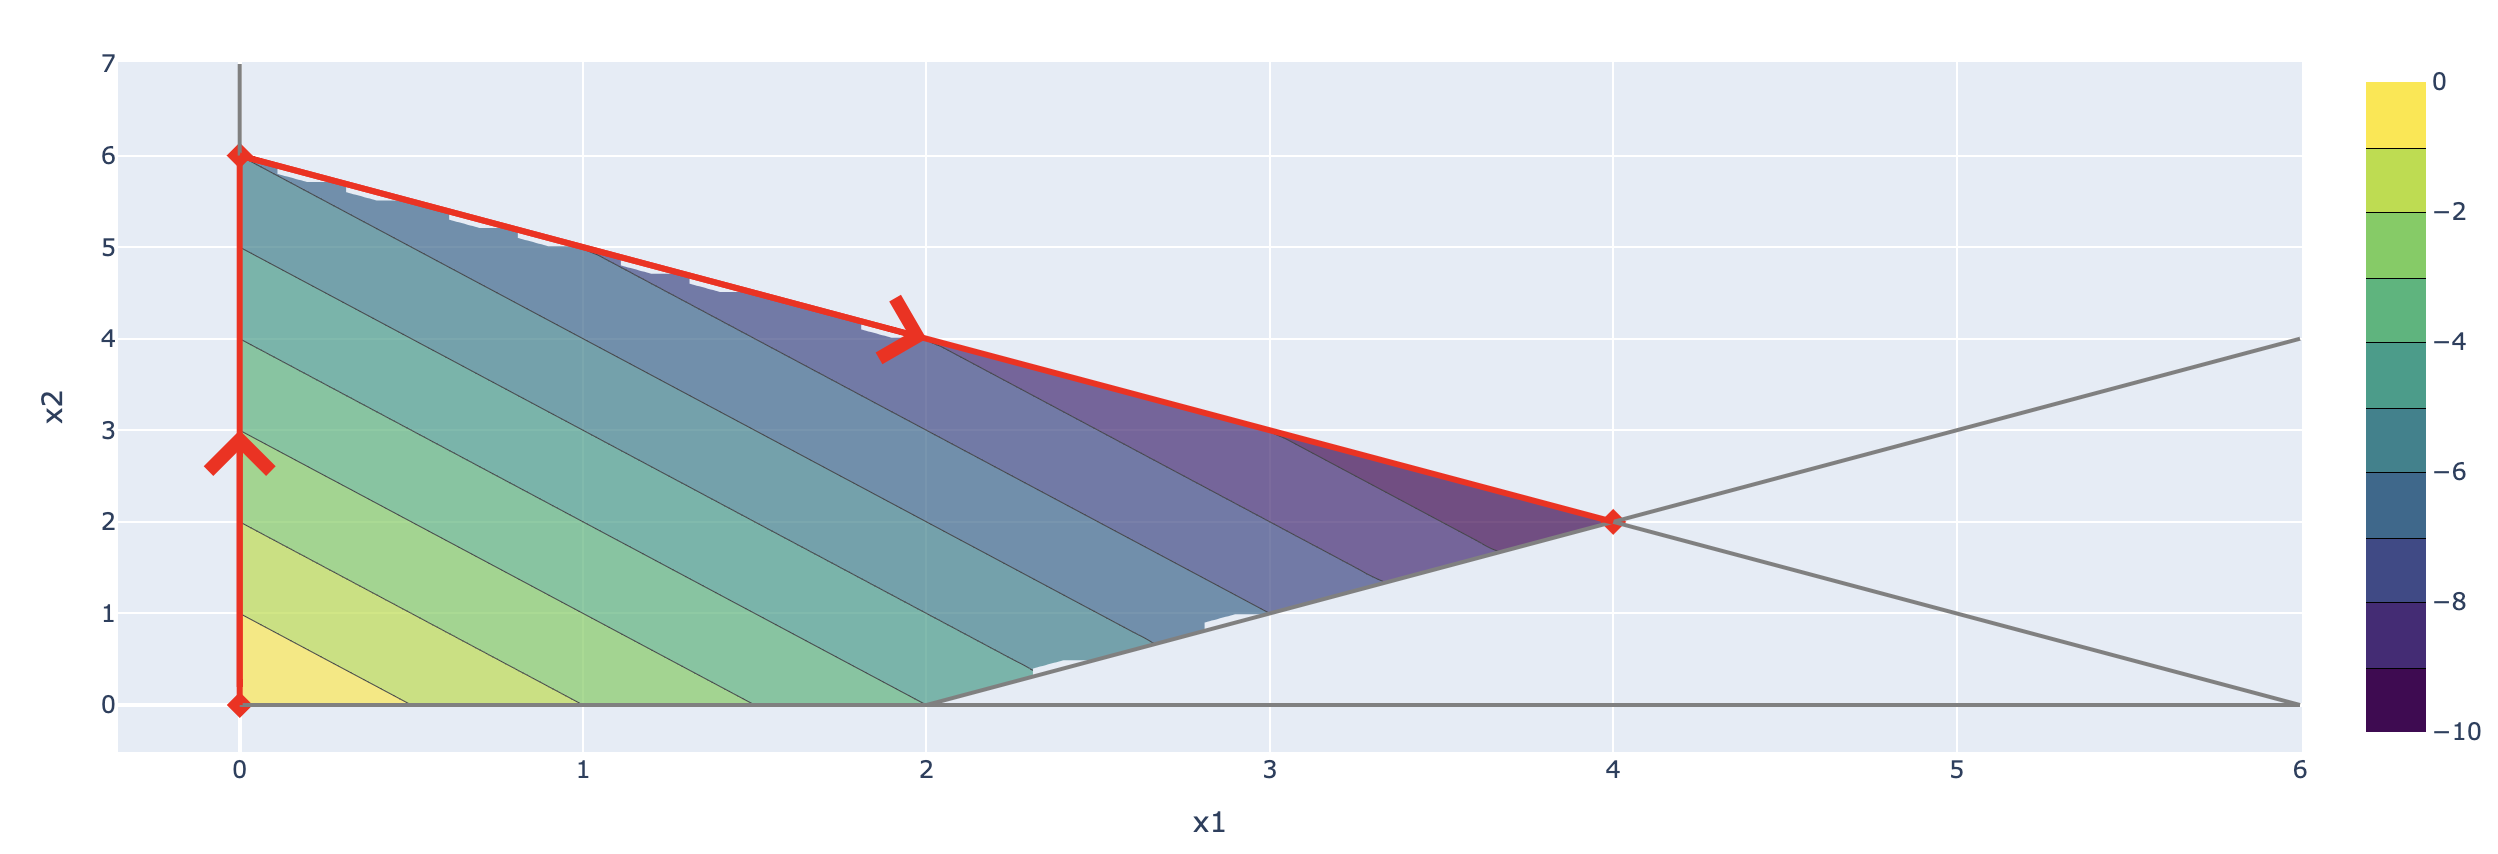
\includegraphics[width=0.9\textwidth]{hw2_problem2c.png}
        \end{center}
        
    \end{parts}

    \question \textbf{3.25 Simplex with upper bound constraint}

    \textbf{Given:}
    \begin{align*}
        \min_x &\quad c^Tx \\
        \text{s.t.} &\quad Ax=b, \quad A \in \mathbb{R}^{m  \times n} \text{ with linearly independent rows}\\
        &\quad 0 \leq x \leq u, \quad u \in \mathbb{R}^n > 0
    \end{align*}
    \begin{parts}
        \part \textbf{Given:} Let $\{B(1), \dots, B(m)\} = B$ be the set of indices of linearly independent columns of $A$. Partition index set $j \notin \{B(1), \dots B(m)\} \in B^C$ into $L, U$. Set $x_j = 0 \quad \forall j \in L$ and set $x_j = u_j \quad \forall j \in U$. Then solve $Ax = b \quad \forall x_i$ for $i \in B$
        \begin{subparts}
            \subpart \label{ref:3.25.a.i}\textbf{Show:} $x$ is a basic solution
            \newline\newline To show $x$ is a basic solution we need to show 
            \newline (A) All equality constraints are active: 
            We start by writing $A = [A_B, A_L, A_U]$ and $x = [x_B, \textbf{0}_L, u_U]^T$ in block form. Since $x_B$ is constructed as the solution to $Ax=b$,
            \begin{align*}
                Ax &= A_Bx_B + A_L\textbf{0} + A_Ux_U = b\\
                x_B &= A_B^{-1}(b - A_Ux_U)
            \end{align*}
            Then we have
            \begin{align*}
                Ax &= A_Bx_B + A_L\textbf{0} + A_Ux_U\\
                &= A_BA_B^{-1}(b - A_Ux_U) + A_Ux_U = b 
            \end{align*}
            So all equality constraints are active
            \newline\newline (B) Of the constraints that are active at x, $n$ are linearly independent. We show this is true by construction. Consider all active constraints in matrix form:
            \begin{align*}
                \begin{bmatrix}
                    A_B & \textbf{0} & \textbf{0}\\
                    \textbf{0} & I_L & \textbf{0}\\
                    \textbf{0}& \textbf{0} & I_U
                \end{bmatrix} \begin{bmatrix}
                    x_B\\ \textbf{0}_L \\ u_U
                \end{bmatrix} = \begin{bmatrix}
                    b \\ \textbf{0}_L \\ u_U
                \end{bmatrix}
            \end{align*}
            Evaluated at $x$, the rows of the LHS matrix of active constraints is block diagonal with diagonal blocks $A_B, I_L, I_U$. These rows are linearly independent if each block is linearly independent. Indeed, block $A_B$ is linearly independent by construction  ($m$ linearly independent columns in an $m \times m$ matrix), as are identity matrices $I_L\in\mathbb{R}^{|L|\times |L|}$ and $I_U \in\mathbb{R}^{|U|\times |U|}$.
            \subpart \textbf{Also show:} $x$ nondegenerate $\iff x_i \neq 0$ and $x_i \neq u_i \quad \forall i \in B$
            \newline(\textbf{Recall:} A basic solution is degenerate if $>n$ (not necessarily linearly independent) constraints are active at $x$)
            \newline\newline \textbf{$\Longrightarrow:$ (Contradiction)} Suppose $\exists i\in B$ such that $x_i = 0$ or $x_i = u_i$. Then we can freely add one more active constraint to the ones identified in part (A), either $e_i^Tx = 0$ or $e_i^Tx = u_i$. This extends the number of equality constraints to $n+1>n$ and hence $x$ is degenerate, which is a contradiction.
            \newline\newline \textbf{$\Longleftarrow:$} Suppose $x_i \neq 0$ and $x_i \neq u_i \quad \forall i \in B$. If so, then the only active constraints are the ones defined in part (A): $Ax = b$, $x_L = 0$, and $x_U = u_U$. These are exactly $n$ constraints and hence $x$ is nondegenerate.
        \end{subparts}
        
        \part \textbf{Given:} $x$ is a basic feasible solution. Let $j$ such that $x_j = 0$ and $\bar c_j < 0$. We adjust the entering and leaving variables: $x_j + \theta^*$ and $x_B - \theta^* B^{-1}A_j$.
        \newline \textbf{Want:} The largest value of $\theta^*$ such that updated $x$ is feasible? How are new basic columns determined?
        \newline\newline We aim to update $x$ to $x + \theta d$, where $\theta > 0$ and search direction $d$ is defined with $d_j = 1$, $d_i = -B^{-1}A_j\; \forall i\in B$, and $d_k = 0$ otherwise. In a standard form polyhedron with only lower bound, $x\geq 0$, the maximum feasible step size is
        \begin{align*}
            \theta^* = \min_{\{i \mid d_i < 0, i\in B\}}\left(-\frac{x_i}{d_i}\right)
        \end{align*}
        This however doesn't guarantee this step size will be feasible since, $\forall i \mid d_i > 0$ this step size will increase $x_i$, possibly with $x_i - \theta d_i > u_i$, violating our upper bound constraint. We therefore have to further control our stepsize with
        \begin{align*}
            \theta^* = \min \left[ \min_{\{i \mid d_i < 0, i\in B\}}\left(- \frac{x_i}{d_i}\right),\quad \min_{\{i \mid d_i > 0, i\in B\}}\left(\frac{u_i - x_i}{d_i}\right)\right]
        \end{align*}
        The exiting variable is the $\arg\min$ of this problem.
        
        
        
        \part \textbf{Given:} $x$ is a basic feasible solution. Let $j$ such that $x_j = u_j$ and $\bar c_j > 0$. We want to adjust the entering and leaving variables: $x_j - \theta^*$ and $x_B + \theta^* B^{-1}A_j$.
        \newline \textbf{Want:} The largest value of $\theta^*$ such that updated $x$ is feasible? How are new basic columns determined?
        \newline\newline By convention that $\theta > 0$, we want to define our search vector, $d$ with  $d_j = -1$, $d_i = B^{-1}A_j\; \forall i\in B$, and $d_k = 0$ otherwise. Again we require $0 \leq x_i \leq u_i$. $d_i > 0 \Rightarrow x_i$ increases and $d_i < 0 \Rightarrow x$ decreases. So with this definition of our search direction, $d$, we arrive at the same definition for $\theta^*$:
        \begin{align*}
            \theta^* = \min \left[ \min_{\{i \mid d_i < 0, i\in B\}}\left(- \frac{x_i}{d_i}\right),\quad \min_{\{i \mid d_i > 0, i\in B\}}\left(\frac{u_i - x_i}{d_i}\right)\right]
        \end{align*}
        Again, the exiting variable is the $argmin$ of this problem.

        
        \part \textbf{Given:} Every basic feasible solution is nondegenerate. 
        \newline \textbf{Show:} the cost strictly decreases with every iteration and the method terminates.
        \newline\newline Intuitively, $\bar c_j$ tells us how much our objective changes when we change $x_j$. When $\bar c_j < 0$, the objective decreases when we increase $x_j$ and when $\bar c_j > 0$, the objective increases when we increase $x_j$. So in our upper+lower bound problem, any $(\bar c_j <0,\; x_j = 0)$ or any $(\bar c_j > 0,\; x_j = u_j)$ are candidate entering variables. 
        \newline\newline Parts (b) and (c) above show us how to construct feasible search directions and step sizes, hence we can define a simplex-like algorithm with a few modifications:
        \begin{itemize}
            \item We consider entering variables $(\bar c_j <0,\; x_j = 0)$ and $(\bar c_j > 0,\; x_j = u_j)$
            \item When the entering variable is $x_j = u_j$, we take the negative of the simplex search direction
            \item We use the feasible step sizes defined in parts (b) and (c)
            \item In every step, our objective decreases by $\theta^* \bar c_j$
        \end{itemize}  
        Since we're given that every basic feasible solution is nondegenerate, this algorithm does not revisit any bases and since there are a finite number of bases, the algorithm will terminate in a finite number of steps. 
    \end{parts}

    
    \question \textbf{3.27 Maximize number of positive components}
    \begin{parts}
        \part \textbf{Want:} $x\in \mathbb{R}^n$ that satisfies $Ax = 0, \; x \geq 0$ with the maximum number of positive components
        \newline \textbf{Show: } This problem can be achieved with
        \begin{align*}
            \max \sum_i y_i\quad s.t. \quad A(z + y) = 0,\; y \leq 1, \; z,y \geq 0
        \end{align*}
        \paragraph{Feasible (z,y):} Begin with any feasible solution $x$ to $Ax = 0,\; x \geq 0$. We can trivially write $x = z + y,\; z,y \geq 0,\; y \leq 1$, demonstrating that for any feasible $x$, we can construct feasible $(z,y)$ for our problem.
        
        \paragraph{Feasible directions:} Our objective value increases in directions that increase $y_i$ (up to 1). Increasing our feasible solution by $ty_i$ increases our objective by $t$, but increases the LHS of our constraint by $tA_i$:
        \begin{align*}
            A(z + y + te_i) = A(z + y) + tA_i = tA_i
        \end{align*}
        We can make a feasible step with $te_i$ if we can also find offsetting $\Delta z$ such that $(z - \Delta z) \geq 0,\; A\Delta z = tA_i$. Then
        \begin{align*}
            A(z -\Delta z + y + te_i) = A(z + y) - A\Delta z + tA_i = -tA_i + tA_i = 0
        \end{align*}
        Now for any $\lambda$ satisfying $A\lambda = 0$, we see $A_i$ can be written as a linear combination of columns $A_{j\neq i}$.
        \begin{align*}
            A\lambda = 0 \Longleftrightarrow \sum_j \lambda_jA_j = 0 \Longleftrightarrow \lambda_iA_i = - \sum_{j\neq i}\lambda_j A_j
        \end{align*}
         When $\lambda_i \neq 0$, we have
        \begin{align*}
            A_i = -\sum_{j\neq i} \frac{\lambda_j}{\lambda_i}A_j
        \end{align*}
        So long as $\exists \lambda$ such that $\lambda_i \neq 0$, then $A_i$ can be written as some linear combination of the other columns of $A$. And in the context of the above problem, we can define
        \begin{align*}
            \Delta z_i = 0,&\quad \Delta z_{j \neq i} = t\frac{\lambda_j}{\lambda_i}\\
            t^* &= \max\{t : t\geq 0,\; y_i + t \leq 1, \; z_j - t\frac{\lambda_j}{\lambda_i} \geq 0 \;\forall j\neq i\} 
        \end{align*}
        To construct feasible direction $e_i - \Delta z$ and step size $t^*$.
        \paragraph{Conic constraint:} Note that our primal problem's constraints form a cone
        \begin{align*}
            x \in \mathcal C = \{x \mid Ax = 0, x \geq 0\}
        \end{align*}
        which means that the feasible solutions are invariant to scaling. i.e., 
        \begin{align*}
            Ax = 0 \Rightarrow A(\alpha x) = \alpha A x = 0 \quad \forall \alpha \in \mathbb{R}
        \end{align*}
        Hence, can we always scale up $(z + y)$ so that $t^* = 1 - y_i$ for feasible index $i$. This means the optimal value to our problem will equal the maximum number of nonzero entries of $x$.
        
        \paragraph{Maximum in finite iterations.} To conclude this proof, observe that any step made in the feasible direction described above improves our objective, specifically by $t*$. Since our problem is a linear program, we are guaranteed to achieve the maximum in a finite number of steps.

        
        \part \textbf{Want:} $x\in \mathbb{R}^n$ that satisfies $Ax = b, \; x \geq 0$ with the maximum number of positive components. \newline\textbf{Show:} This problem can be achieved with a linear program.
        \paragraph{Proposed linear program:}
        \begin{align*}
            \max_{z, y, \theta} \quad& \sum_i y_i\\
            s.t.\quad& A(z + y) = \theta b\\
            & y \leq 1, \; z,y,\theta \geq 0
        \end{align*}

        \paragraph{Feasible $(z,y,\theta)$:} Begin with any feasible solution $x$ to $Ax = b,\; x \geq 0$. We can trivially select $z,y,\theta \geq 0,\; y \leq 1$ such that $\theta x = (z + y)$, so
        \begin{align*}
            A(z + y) = A(\theta x) = \theta Ax = \theta b
        \end{align*}
        Demonstrating that for any feasible $x$, we can construct feasible $(z,y,\theta)$ for our problem.
        
        \paragraph{Feasible directions:} As in part (a), we can increase our objective function by $t$ by increasing our feasible solution by $te_i$, so long as we can find offsetting shifts to stay feasible. 
        \begin{align*}
            A(z - t\Delta z +y+te_i) = (\theta + t\Delta \theta) b \text{, feasible if } \exists \; \Delta z, \Delta\theta \text{ s.t. } A_i = A\Delta z + \Delta \theta b
        \end{align*}
        This is an equivalent problem to our original search for $\Delta z$ in part (a), only lifted to $\mathbb{R}^{n+1}$. We can increase the value of $y_i$ so long as we can find any such vector $[\Delta z, \Delta \theta]^T$ such that $A_i$ can be written as a linear combination of the columns of $[A, b]$ 
        \paragraph{Conic constraint:} Our new equality constraint lifted into $(x, \theta)$ space is also a cone constraint. Specifically, if point $(z, y, \theta)$ is scaled by $\alpha > 0$, the new point is still feasible:
        \begin{align*}
            A(\alpha z + \alpha y) = \alpha A(z + y) = \alpha \theta b
        \end{align*}
        Hence, as in part (a), any feasible point can be scaled up so that all positive $y_i$ reach their upper bound of $1$. Therefore, the optimal value of our linear program equals the maximum number of positive components of any feasible $x$ satisfying $Ax = b,\; x \geq 0$.
        
    \end{parts}
    \question \textbf{Simplex implementation and solutions}
    \paragraph{Solutions.}
    \begin{minted}[fontsize=\small]{text}
==== problem 1 ====
---- part 1 ----
Phase 1 simplex - find BFS
	status:	 optimal
	opt. value:	 0.0
Phase 2 simplex - optimize
	status:	optimal
	opt. value:	 4.0499
---- part 2 ----
    \end{minted}
    \begin{center}
        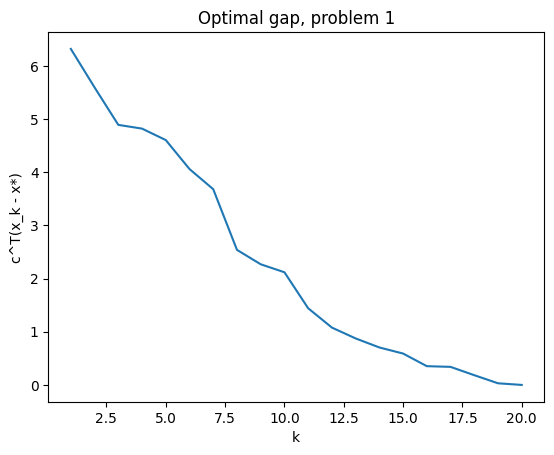
\includegraphics[width=0.75\textwidth]{hw2_problem5_2_1.png}
    \end{center}


\begin{minted}[fontsize=\small]{text}
==== problem 2 ====
---- part 1 ----
Phase 1 simplex - find BFS
	status:	   optimal
	opt. value:	 3.1735
Phase 2 simplex skipped - infeasible
	status:	infeasible
	opt. value:	 None
---- part 2 ----
No iterations to show


==== problem 3 ====
---- part 1 ----
Phase 1 simplex - find BFS
	status:	optimal
	opt. value:	 0.0
Phase 2 simplex - optimize
	status:	unbounded
	opt. value:	 None
---- part 2 ----
No iterations to show
    \end{minted}
    \paragraph{Code.}
    \begin{minted}[fontsize=\tiny, breaklines, linenos]{python}
import numpy as np
import os
from typing import Tuple

# read in data
dir = os.getcwd()
def get_data(problem):
    A = np.loadtxt(f"{dir}/data/hw2_data/{problem}/A.csv", delimiter=",")
    b = np.loadtxt(f"{dir}/data/hw2_data/{problem}/b.csv", delimiter=",")
    c = np.loadtxt(f"{dir}/data/hw2_data/{problem}/c.csv", delimiter=",")
    return A, b, c

# Simplex with a given BFS
def simplex_w_bfs(
        A, b, c, x_bfs, eps = 1e-10, max_iter = 200
    ) -> Tuple[str, np.ndarray | None, np.ndarray | None]:
    x_i = x_bfs
    x_is = [x_i.copy()]
    for i in range(max_iter):
        # -1- step 1: initialize variables
        B = x_i > 0
        A_B_inv = np.linalg.inv(A[:, B])
        u = A_B_inv @ A
        # -2- step 2: calculate cost difference
        c_bar = c - c[B] @ u
        c_bar[np.abs(c_bar) < eps] = 0
        # CHECK: return optimal if cbar > 0
        if np.all(c_bar >= 0):
            return "optimal", x_i, np.array(x_is)
        # -3- step 3: choose entering variable
        e = int(np.where(c_bar < 0)[0][0]) # first negative
        e = int(np.argmin(c_bar)) # most negative
        d = np.zeros(x_i.shape[0])
        d[e] = 1
        d[B] = -u[:, e]
        # CHECK: return unbounded if d >= 0
        if np.all(d >= 0):
            return "unbounded", None, None
        # -4- step 4: compute greedy step size
        S = (d < 0) & B
        theta = np.min(x_i[S] / -d[S])
        x_i += theta * d
        x_i[np.abs(x_i) < eps] = 0
        x_is += [x_i.copy()]
    return "max_iter", x_i, np.array(x_is)

# Two-phase simplex
def simplex_2phase(A, b, c) -> Tuple[str, np.ndarray | None, np.ndarray | None]:
    # -A- Initialize Phase 1
    A_p = np.concatenate([A, np.eye(A.shape[0])], axis=1)
    A_p[b < 0, :A.shape[1]] *= -1
    b_p = np.abs(b)
    c_p = np.concat([np.zeros(c.shape[0]), np.ones(b.shape[0])])
    xy_bfs = np.concat([np.zeros(A.shape[1]), b_p])
    # check:
    assert np.allclose(A_p @ xy_bfs, b_p)
    
    # -B- Phase 1
    print("Phase 1 simplex - find BFS")
    status, xy_opt, __ = simplex_w_bfs(A_p, b_p, c_p, xy_bfs)
    print(f"\tstatus:\t\t {status}")
    print(f"\topt. value:\t {np.round(c_p @ xy_opt, 4) if xy_opt is not None else None}")
    # check:
    if (c_p @ xy_opt) > 1e-5:
        print("Phase 2 simplex skipped - infeasible")
        print("\tstatus:\t\t infeasible")
        print("\topt. value:\t None")
        return "infeasible", None, None

    # -C- Phase 2
    x_bfs = xy_opt[:A.shape[1]]
    print("Phase 2 simplex - optimize")
    status, x_opt, x_is = simplex_w_bfs(A, b, c, x_bfs)
    print(f"\tstatus:\t\t {status}")
    print(f"\topt. value:\t {np.round(c @ x_opt, 4) if x_opt is not None else None}")
    return status, x_opt, x_is
    \end{minted}

\end{questions}
\end{document}